\documentclass[hidelinks,12pt,dvipsnames,border=2pt]{standalone}
%\usepackage[top=0.7in, bottom=0.8in, left=1in, right=1in]{geometry}
\usepackage{tikz}
\usepackage{hyperref}
\usetikzlibrary{arrows}
\usetikzlibrary{shapes}
\usepackage{enumitem}
\usepackage{bm}
\usepackage{mathdots}
\usepackage{amsmath}
\usepackage{tcolorbox}
\usetikzlibrary{shadings}
\usetikzlibrary{decorations.pathreplacing}
\usepackage{helvet}
\usepackage{url}
\usepackage{graphicx}
\usetikzlibrary{arrows.meta,positioning,fit,calc}
\renewcommand{\familydefault}{\sfdefault}

\definecolor{p1}{HTML}{440154}
\definecolor{p2}{HTML}{482576}
\definecolor{p3}{HTML}{414487}
\definecolor{p4}{HTML}{35608D}
\definecolor{p5}{HTML}{2A788E}
\definecolor{p6}{HTML}{21908C}
\definecolor{p7}{HTML}{22A884}
\definecolor{p8}{HTML}{43BF71}
\definecolor{p9}{HTML}{7AD151}
\usetikzlibrary{arrows,decorations.pathmorphing,backgrounds,fit,positioning,shapes.symbols,chains}

\begin{document}
	
% trim=left botm right top
\begin{tikzpicture}

\node at (0,0) {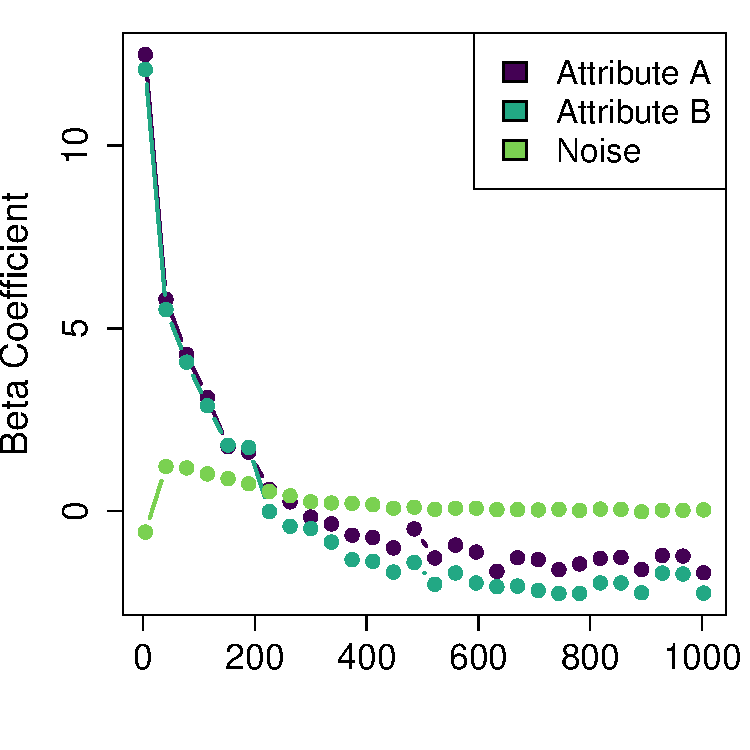
\includegraphics[width=\textwidth]{betas_vs_p_ABC.pdf}};
\node at (13.75,0) {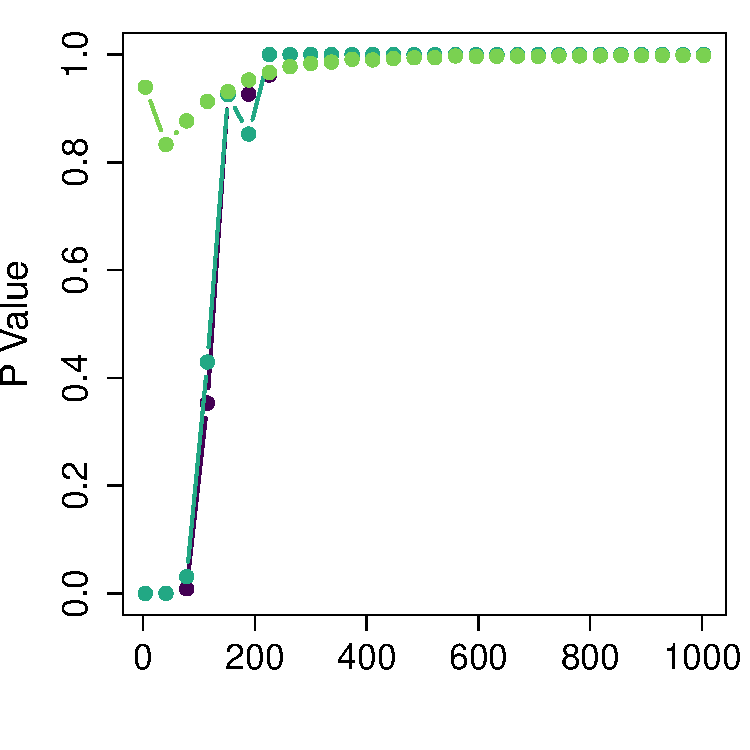
\includegraphics[width=\textwidth]{pvals_vs_p_ABC.pdf}};

%\node[xscale=1.9,yscale=1.9] at (0.85,7) {Standard Normal Data};
%\node[xscale=1.9,yscale=1.9] at (13.6,7) {Standard Uniform Data};

\node[xscale=2.2,yscale=2.2] at (-6.54,6.1) {\fontfamily{ptm}\selectfont \textbf{I}};
\node[xscale=2.2,yscale=2.2] at (7.21,6.1) {\fontfamily{ptm}\selectfont \textbf{II}};

\node[xscale=1.6,yscale=1.6] at (7.9,-6.4) {Number of Attributes ($p$)};

\end{tikzpicture}

\end{document}